\section{Results}
\label{sec:results}

%% FIGURE: Visual comparison of controller performance for the block M.
\begin{figure*}
    \centering
    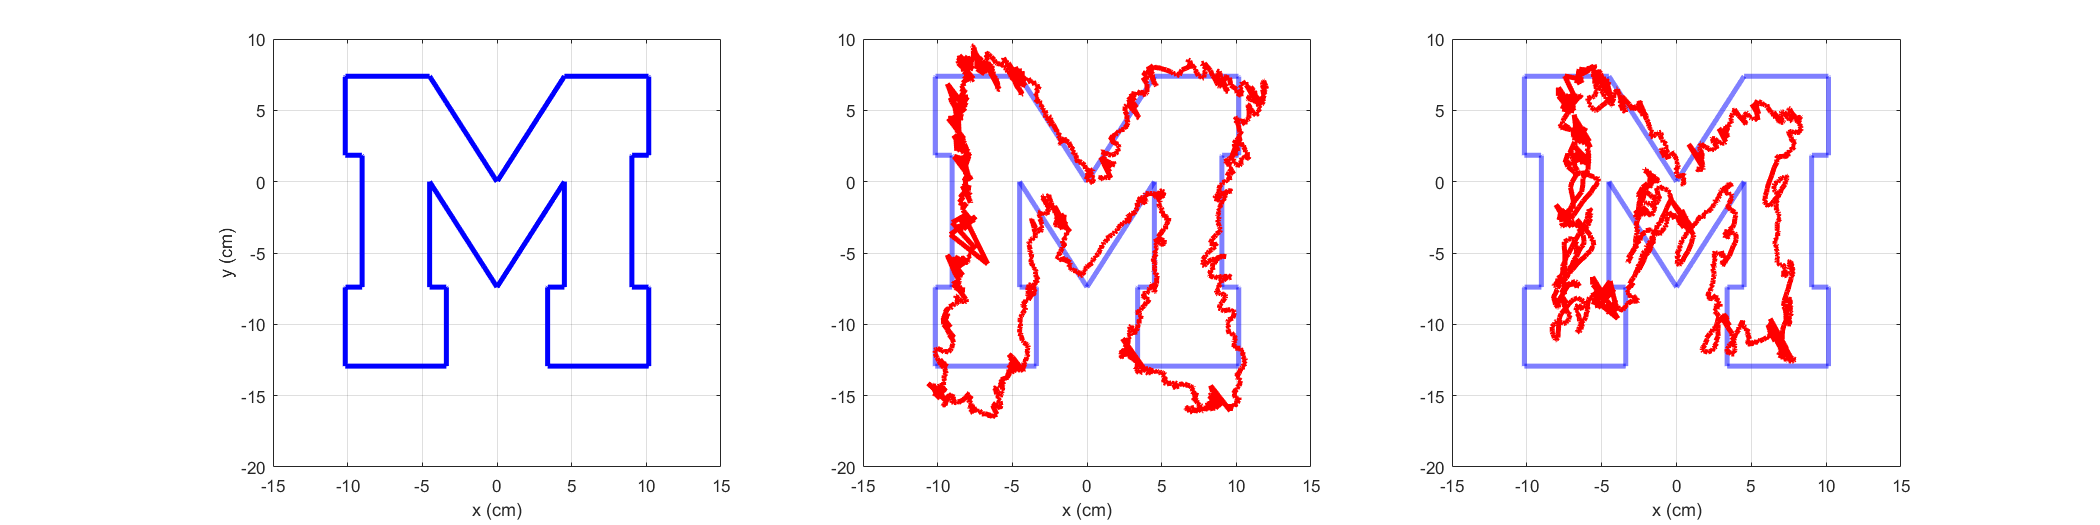
\includegraphics[width=\linewidth]{figures/compare_blockM_300s_draft.png}
    \caption{The results of each controller to performing task 1. Reference trajectory only (left). Koopman MPC (middle). Linear MPC (right). Laser dot trajectory is shown in red, the reference trajectory is shown in blue.}
    \label{fig:compare_blockM}
\end{figure*}

%% FIGURE: Visual comparison of controller performance for the pacman.
\begin{figure*}
    \centering
    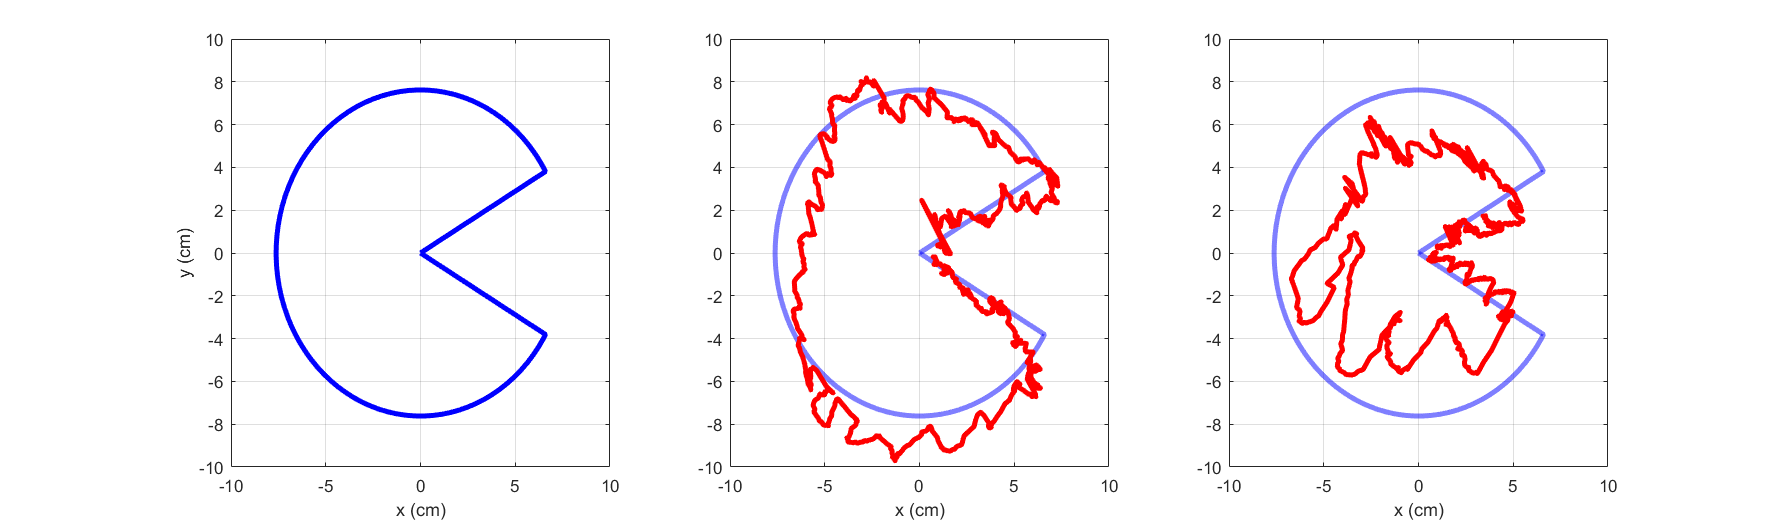
\includegraphics[width=\linewidth]{figures/compare_pacman68_90s_draft.png}
    \caption{The results of each controller to performing task 2. Reference trajectory only (left). Koopman MPC (middle). Linear MPC (right). Laser dot trajectory is shown in red, the reference trajectory is shown in blue.}
    \label{fig:compare_pacman}
\end{figure*}

%% TABLE: RMSE results table
\begin{table}[]
    \rowcolors{2}{white}{gray!25}
    \setlength\tabcolsep{5pt} % default value: 6pt
    \centering
    \caption{RMSE (cm) over all trajectory following tasks \Dan{Fill in real results later}}
    \begin{tabular}{|c|c|c|c|c|c|c|c|c|}
        \hline
        \rowcolor{white} 
        & \multicolumn{6}{c |}{\textbf{Task}} & & \textbf{Std.} \\
        \cline{2-7} \rowcolor{white}
        \multirow{-2}{*}{\textbf{Controller}} & $1$ & $2$ & $3$ & $4$ & $5$ & $6$ & \multirow{-2}{*}{\textbf{Avg.}} & \textbf{Dev.} \\
        \hline
        % RESULTS FOR ROBOT A
        Koopman MPC &  2.4  &  2.0  &  2.9  &  1.7  &  1.5  &  2.0 & 2.1 & 0.5 \\
        Linear MPC  &  5.8  &  4.0  &  6.6  &  3.9  &  2.8  &  3.5 & 4.5 & 1.5 \\
        Nonlinear MPC &  5.1  &  3.1  &  9.9  &  3.0  &  1.8  &  4.8 & 4.6 & 2.9 \\
        % Ham.-Weiner &  7.0  &  4.5  &  6.9  &  3.0  &  2.3  &  3.1 & 4.5 & 2.0 \\
        % \multirow{-5}{*}{\cellcolor{white} \rotatebox[origin=c]{90}{\textbf{Robot A}}}
        % NLARX       &  5.0  &  3.0 &  12.0  &  3.8  &  2.1  &  2.8 & 4.8 & 3.7 \\
        \hline
        % % RESULTS FOR ROBOT B
        % \cellcolor{white} & Koopman & & & & & & & & \\
        % \cellcolor{white} & Neural Net & & & & & & & & \\
        % \cellcolor{white} & State Space & & & & & & & & \\
        % \cellcolor{white} & Ham.-Weiner & & & & & & & & \\
        % \multirow{-5}{*}{\cellcolor{white} \rotatebox[origin=c]{90}{\textbf{Robot B}}}
        % & NLARX & & & & & & & & \\
        % \hline
    \end{tabular}
    \label{tab:RMSE}
\end{table}
